\documentclass[a4paper,12pt]{article}
\usepackage[margin=18mm]{geometry}
\usepackage{tikz}
\usepackage{amsmath}
\usepackage{xcolor}
\newcommand{\pFourCell}[2]{\makebox[#1em][c]{\ensuremath{#2}}}
\newdimen\pFourFractionRuleThickness
\pFourFractionRuleThickness=0.4pt
\newcommand{\pFourFractionC}[4]{\begingroup\setbox0=\hbox{$\displaystyle #3$}\setbox2=\hbox{$\displaystyle #4$}\dimen0=\ht0\advance\dimen0 by \dp0\advance\dimen0 by 0.14em\dimen2=\ht2\advance\dimen2 by \dp2\advance\dimen2 by 0.18em\dimen4=\pFourFractionRuleThickness\divide\dimen4 by 2\advance\dimen0 by \dimen4\advance\dimen2 by \dimen4\dimen6=\dimen0\advance\dimen6 by -\dimen2\divide\dimen6 by 2\lower\dimen6\hbox{$\vcenter{\offinterlineskip\halign{##\cr\hbox to #2{\hss$\displaystyle #3$\hss}\cr\noalign{\kern0.14em{\color{#1}\hrule height \pFourFractionRuleThickness width #2}\kern0.18em}\hbox to #2{\hss$\displaystyle #4$\hss}\cr}}$}\endgroup}
\newcommand{\pFourFraction}[3]{\begingroup\setbox0=\hbox{$\displaystyle #2$}\setbox2=\hbox{$\displaystyle #3$}\dimen0=\ht0\advance\dimen0 by \dp0\advance\dimen0 by 0.14em\dimen2=\ht2\advance\dimen2 by \dp2\advance\dimen2 by 0.18em\dimen4=\pFourFractionRuleThickness\divide\dimen4 by 2\advance\dimen0 by \dimen4\advance\dimen2 by \dimen4\dimen6=\dimen0\advance\dimen6 by -\dimen2\divide\dimen6 by 2\lower\dimen6\hbox{$\vcenter{\offinterlineskip\halign{##\cr\hbox to #1{\hss$\displaystyle #2$\hss}\cr\noalign{\kern0.14em\hrule height \pFourFractionRuleThickness width #1\kern0.18em}\hbox to #1{\hss$\displaystyle #3$\hss}\cr}}$}\endgroup}
\newcommand{\pFourRootC}[2]{\begingroup\setbox0=\hbox{$\displaystyle #2$}\setbox2=\hbox{$\displaystyle \sqrt{\vphantom{\copy0}\hphantom{\copy0}}$}\dimen0=\wd2\advance\dimen0 by -\wd0\hbox{\rlap{\textcolor{#1}{\copy2}}\kern\dimen0\box0}\endgroup}
\newcommand{\pFourRoot}[1]{\pFourRootC{black}{#1}}
\pagestyle{empty}
\begin{document}

\section*{Spaltentreue LaTeX-Ausgabe}
\noindent Gleichung: \texttt{sin}\texttt{(}\ensuremath{\alpha}\texttt{)/}\texttt{a}\texttt{=}\texttt{b}\texttt{/}\texttt{sin}\texttt{(}\ensuremath{\beta}\texttt{)} \hfill Zielvariable: \texttt{a} \hfill Profil: \texttt{standard}

\vspace{8mm}
\begin{center}
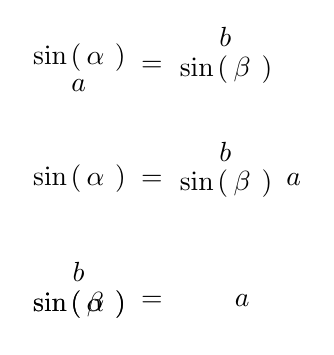
\begin{tikzpicture}[x=1em,y=-1em]
\node[anchor=base, inner sep=0pt] at (1.84,2.59) {$\pFourFraction{3.68em}{\pFourCell{1.62}{\sin}\pFourCell{0.38}{\left(\vphantom{\pFourCell{0.9}{\alpha}}\right.}\pFourCell{0.9}{\alpha}\pFourCell{0.78}{\left.\vphantom{\pFourCell{0.9}{\alpha}}\right)}}{\makebox[3.68em][c]{\ensuremath{\pFourCell{0.9}{a}}}}$};
\node[anchor=base, inner sep=0pt] at (7.14,2.59) {$\pFourFraction{3.68em}{\makebox[3.68em][c]{\ensuremath{\pFourCell{0.9}{b}}}}{\pFourCell{1.62}{\sin}\pFourCell{0.38}{\left(\vphantom{\pFourCell{0.9}{\beta}}\right.}\pFourCell{0.9}{\beta}\pFourCell{0.78}{\left.\vphantom{\pFourCell{0.9}{\beta}}\right)}}$};
\node[anchor=base, inner sep=0pt] at (4.49,2.73) {$\pFourCell{1.62}{=}$};
\node[anchor=base, inner sep=0pt] at (7.14,6.72) {$\pFourFraction{3.68em}{\makebox[3.68em][c]{\ensuremath{\pFourCell{0.9}{b}}}}{\pFourCell{1.62}{\sin}\pFourCell{0.38}{\left(\vphantom{\pFourCell{0.9}{\beta}}\right.}\pFourCell{0.9}{\beta}\pFourCell{0.78}{\left.\vphantom{\pFourCell{0.9}{\beta}}\right)}}$};
\node[anchor=base, inner sep=0pt] at (2.45,6.86) {$\pFourCell{0.9}{\alpha}$};
\node[anchor=base, inner sep=0pt] at (0.81,6.86) {$\pFourCell{1.62}{\sin}$};
\node[anchor=base, inner sep=0pt] at (1.81,6.86) {$\pFourCell{0.38}{\left(\vphantom{\pFourCell{0.9}{\alpha}}\right.}$};
\node[anchor=base, inner sep=0pt] at (3.29,6.86) {$\pFourCell{0.78}{\left.\vphantom{\pFourCell{0.9}{\alpha}}\right)}$};
\node[anchor=base, inner sep=0pt] at (4.49,6.86) {$\pFourCell{1.62}{=}$};
\node[anchor=base, inner sep=0pt] at (9.61,6.86) {$\pFourCell{0.9}{a}$};
\node[anchor=base, inner sep=0pt] at (1.84,11.09) {$\pFourFraction{3.68em}{\pFourCell{1.62}{\sin}\pFourCell{0.38}{\left(\vphantom{\pFourCell{0.9}{\alpha}}\right.}\pFourCell{0.9}{\alpha}\pFourCell{0.78}{\left.\vphantom{\pFourCell{0.9}{\alpha}}\right)}}{\makebox[3.68em][c]{\ensuremath{}}}$};
\node[anchor=base, inner sep=0pt] at (1.84,11.07) {$\pFourFraction{3.68em}{\makebox[3.68em][c]{\ensuremath{\pFourCell{0.9}{b}}}}{\pFourCell{1.62}{\sin}\pFourCell{0.38}{\left(\vphantom{\pFourCell{0.9}{\beta}}\right.}\pFourCell{0.9}{\beta}\pFourCell{0.78}{\left.\vphantom{\pFourCell{0.9}{\beta}}\right)}}$};
\node[anchor=base, inner sep=0pt] at (4.49,11.23) {$\pFourCell{1.62}{=}$};
\node[anchor=base, inner sep=0pt] at (7.75,11.23) {$\pFourCell{0.9}{a}$};
\end{tikzpicture}
\end{center}


\newpage
\section*{Spaltentreue LaTeX-Ausgabe mit Spaltengrenzen}
\vspace{6mm}
\begin{center}
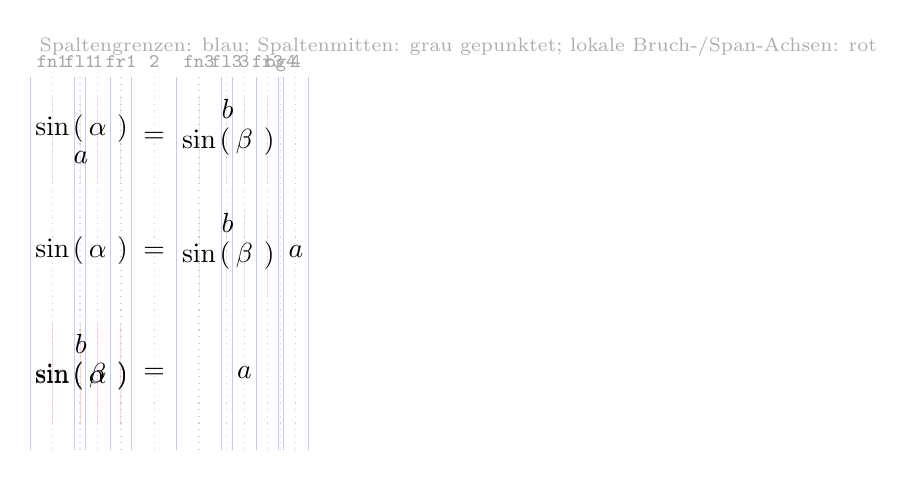
\begin{tikzpicture}[x=1em,y=-1em]
\node[font={\scriptsize}, text=gray!65, anchor=west] at (0,-0.75) {Spaltengrenzen: blau; Spaltenmitten: grau gepunktet; lokale Bruch-/Span-Achsen: rot};
\draw[blue!22, line width=0.28pt] (0,0.35) -- (0,13.82);
\draw[blue!22, line width=0.28pt] (1.62,0.35) -- (1.62,13.82);
\draw[blue!22, line width=0.28pt] (2,0.35) -- (2,13.82);
\draw[blue!22, line width=0.28pt] (2.9,0.35) -- (2.9,13.82);
\draw[blue!22, line width=0.28pt] (3.68,0.35) -- (3.68,13.82);
\draw[blue!22, line width=0.28pt] (5.3,0.35) -- (5.3,13.82);
\draw[blue!22, line width=0.28pt] (6.92,0.35) -- (6.92,13.82);
\draw[blue!22, line width=0.28pt] (7.3,0.35) -- (7.3,13.82);
\draw[blue!22, line width=0.28pt] (8.2,0.35) -- (8.2,13.82);
\draw[blue!22, line width=0.28pt] (8.98,0.35) -- (8.98,13.82);
\draw[blue!22, line width=0.28pt] (9.16,0.35) -- (9.16,13.82);
\draw[blue!22, line width=0.28pt] (10.06,0.35) -- (10.06,13.82);
\draw[gray!35, dotted] (0.81,0.35) -- (0.81,13.82);
\node[font={\ttfamily\scriptsize}, text=gray!70, anchor=base] at (0.81,0) {fn1};
\draw[gray!35, dotted] (1.81,0.35) -- (1.81,13.82);
\node[font={\ttfamily\scriptsize}, text=gray!70, anchor=base] at (1.81,0) {fl1};
\draw[gray!35, dotted] (2.45,0.35) -- (2.45,13.82);
\node[font={\ttfamily\scriptsize}, text=gray!70, anchor=base] at (2.45,0) {1};
\draw[gray!35, dotted] (3.29,0.35) -- (3.29,13.82);
\node[font={\ttfamily\scriptsize}, text=gray!70, anchor=base] at (3.29,0) {fr1};
\draw[gray!35, dotted] (4.49,0.35) -- (4.49,13.82);
\node[font={\ttfamily\scriptsize}, text=gray!70, anchor=base] at (4.49,0) {2};
\draw[gray!35, dotted] (6.11,0.35) -- (6.11,13.82);
\node[font={\ttfamily\scriptsize}, text=gray!70, anchor=base] at (6.11,0) {fn3};
\draw[gray!35, dotted] (7.11,0.35) -- (7.11,13.82);
\node[font={\ttfamily\scriptsize}, text=gray!70, anchor=base] at (7.11,0) {fl3};
\draw[gray!35, dotted] (7.75,0.35) -- (7.75,13.82);
\node[font={\ttfamily\scriptsize}, text=gray!70, anchor=base] at (7.75,0) {3};
\draw[gray!35, dotted] (8.59,0.35) -- (8.59,13.82);
\node[font={\ttfamily\scriptsize}, text=gray!70, anchor=base] at (8.59,0) {fr3};
\draw[gray!35, dotted] (9.07,0.35) -- (9.07,13.82);
\node[font={\ttfamily\scriptsize}, text=gray!70, anchor=base] at (9.07,0) {bg4};
\draw[gray!35, dotted] (9.61,0.35) -- (9.61,13.82);
\node[font={\ttfamily\scriptsize}, text=gray!70, anchor=base] at (9.61,0) {4};
\draw[red!30, opacity=0.32, line width=0.35pt] (0.81,1) -- (0.81,4.18);
\draw[red!30, opacity=0.32, line width=0.35pt] (1.81,1) -- (1.81,4.18);
\draw[red!30, opacity=0.32, line width=0.35pt] (2.45,1) -- (2.45,4.18);
\draw[red!30, opacity=0.32, line width=0.35pt] (3.29,1) -- (3.29,4.18);
\node[anchor=base, inner sep=0pt] at (1.84,2.59) {$\pFourFraction{3.68em}{\pFourCell{1.62}{\sin}\pFourCell{0.38}{\left(\vphantom{\pFourCell{0.9}{\alpha}}\right.}\pFourCell{0.9}{\alpha}\pFourCell{0.78}{\left.\vphantom{\pFourCell{0.9}{\alpha}}\right)}}{\makebox[3.68em][c]{\ensuremath{\pFourCell{0.9}{a}}}}$};
\draw[red!30, opacity=0.32, line width=0.35pt] (6.11,1) -- (6.11,4.18);
\draw[red!30, opacity=0.32, line width=0.35pt] (7.11,1) -- (7.11,4.18);
\draw[red!30, opacity=0.32, line width=0.35pt] (7.75,1) -- (7.75,4.18);
\draw[red!30, opacity=0.32, line width=0.35pt] (8.59,1) -- (8.59,4.18);
\node[anchor=base, inner sep=0pt] at (7.14,2.59) {$\pFourFraction{3.68em}{\makebox[3.68em][c]{\ensuremath{\pFourCell{0.9}{b}}}}{\pFourCell{1.62}{\sin}\pFourCell{0.38}{\left(\vphantom{\pFourCell{0.9}{\beta}}\right.}\pFourCell{0.9}{\beta}\pFourCell{0.78}{\left.\vphantom{\pFourCell{0.9}{\beta}}\right)}}$};
\node[anchor=base, inner sep=0pt] at (4.49,2.73) {$\pFourCell{1.62}{=}$};
\draw[red!30, opacity=0.32, line width=0.35pt] (6.11,5.13) -- (6.11,8.31);
\draw[red!30, opacity=0.32, line width=0.35pt] (7.11,5.13) -- (7.11,8.31);
\draw[red!30, opacity=0.32, line width=0.35pt] (7.75,5.13) -- (7.75,8.31);
\draw[red!30, opacity=0.32, line width=0.35pt] (8.59,5.13) -- (8.59,8.31);
\node[anchor=base, inner sep=0pt] at (7.14,6.72) {$\pFourFraction{3.68em}{\makebox[3.68em][c]{\ensuremath{\pFourCell{0.9}{b}}}}{\pFourCell{1.62}{\sin}\pFourCell{0.38}{\left(\vphantom{\pFourCell{0.9}{\beta}}\right.}\pFourCell{0.9}{\beta}\pFourCell{0.78}{\left.\vphantom{\pFourCell{0.9}{\beta}}\right)}}$};
\node[anchor=base, inner sep=0pt] at (2.45,6.86) {$\pFourCell{0.9}{\alpha}$};
\node[anchor=base, inner sep=0pt] at (0.81,6.86) {$\pFourCell{1.62}{\sin}$};
\node[anchor=base, inner sep=0pt] at (1.81,6.86) {$\pFourCell{0.38}{\left(\vphantom{\pFourCell{0.9}{\alpha}}\right.}$};
\node[anchor=base, inner sep=0pt] at (3.29,6.86) {$\pFourCell{0.78}{\left.\vphantom{\pFourCell{0.9}{\alpha}}\right)}$};
\node[anchor=base, inner sep=0pt] at (4.49,6.86) {$\pFourCell{1.62}{=}$};
\node[anchor=base, inner sep=0pt] at (9.61,6.86) {$\pFourCell{0.9}{a}$};
\draw[red!30, opacity=0.32, line width=0.35pt] (0.81,9.26) -- (0.81,12.92);
\draw[red!30, opacity=0.32, line width=0.35pt] (1.81,9.26) -- (1.81,12.92);
\draw[red!30, opacity=0.32, line width=0.35pt] (2.45,9.26) -- (2.45,12.92);
\draw[red!30, opacity=0.32, line width=0.35pt] (3.29,9.26) -- (3.29,12.92);
\node[anchor=base, inner sep=0pt] at (1.84,11.09) {$\pFourFraction{3.68em}{\pFourCell{1.62}{\sin}\pFourCell{0.38}{\left(\vphantom{\pFourCell{0.9}{\alpha}}\right.}\pFourCell{0.9}{\alpha}\pFourCell{0.78}{\left.\vphantom{\pFourCell{0.9}{\alpha}}\right)}}{\makebox[3.68em][c]{\ensuremath{}}}$};
\draw[red!30, opacity=0.32, line width=0.35pt] (0.81,9.26) -- (0.81,12.92);
\draw[red!30, opacity=0.32, line width=0.35pt] (1.81,9.26) -- (1.81,12.92);
\draw[red!30, opacity=0.32, line width=0.35pt] (2.45,9.26) -- (2.45,12.92);
\draw[red!30, opacity=0.32, line width=0.35pt] (3.29,9.26) -- (3.29,12.92);
\node[anchor=base, inner sep=0pt] at (1.84,11.07) {$\pFourFraction{3.68em}{\makebox[3.68em][c]{\ensuremath{\pFourCell{0.9}{b}}}}{\pFourCell{1.62}{\sin}\pFourCell{0.38}{\left(\vphantom{\pFourCell{0.9}{\beta}}\right.}\pFourCell{0.9}{\beta}\pFourCell{0.78}{\left.\vphantom{\pFourCell{0.9}{\beta}}\right)}}$};
\node[anchor=base, inner sep=0pt] at (4.49,11.23) {$\pFourCell{1.62}{=}$};
\node[anchor=base, inner sep=0pt] at (7.75,11.23) {$\pFourCell{0.9}{a}$};
\end{tikzpicture}
\end{center}
\end{document}
